\begin{center}
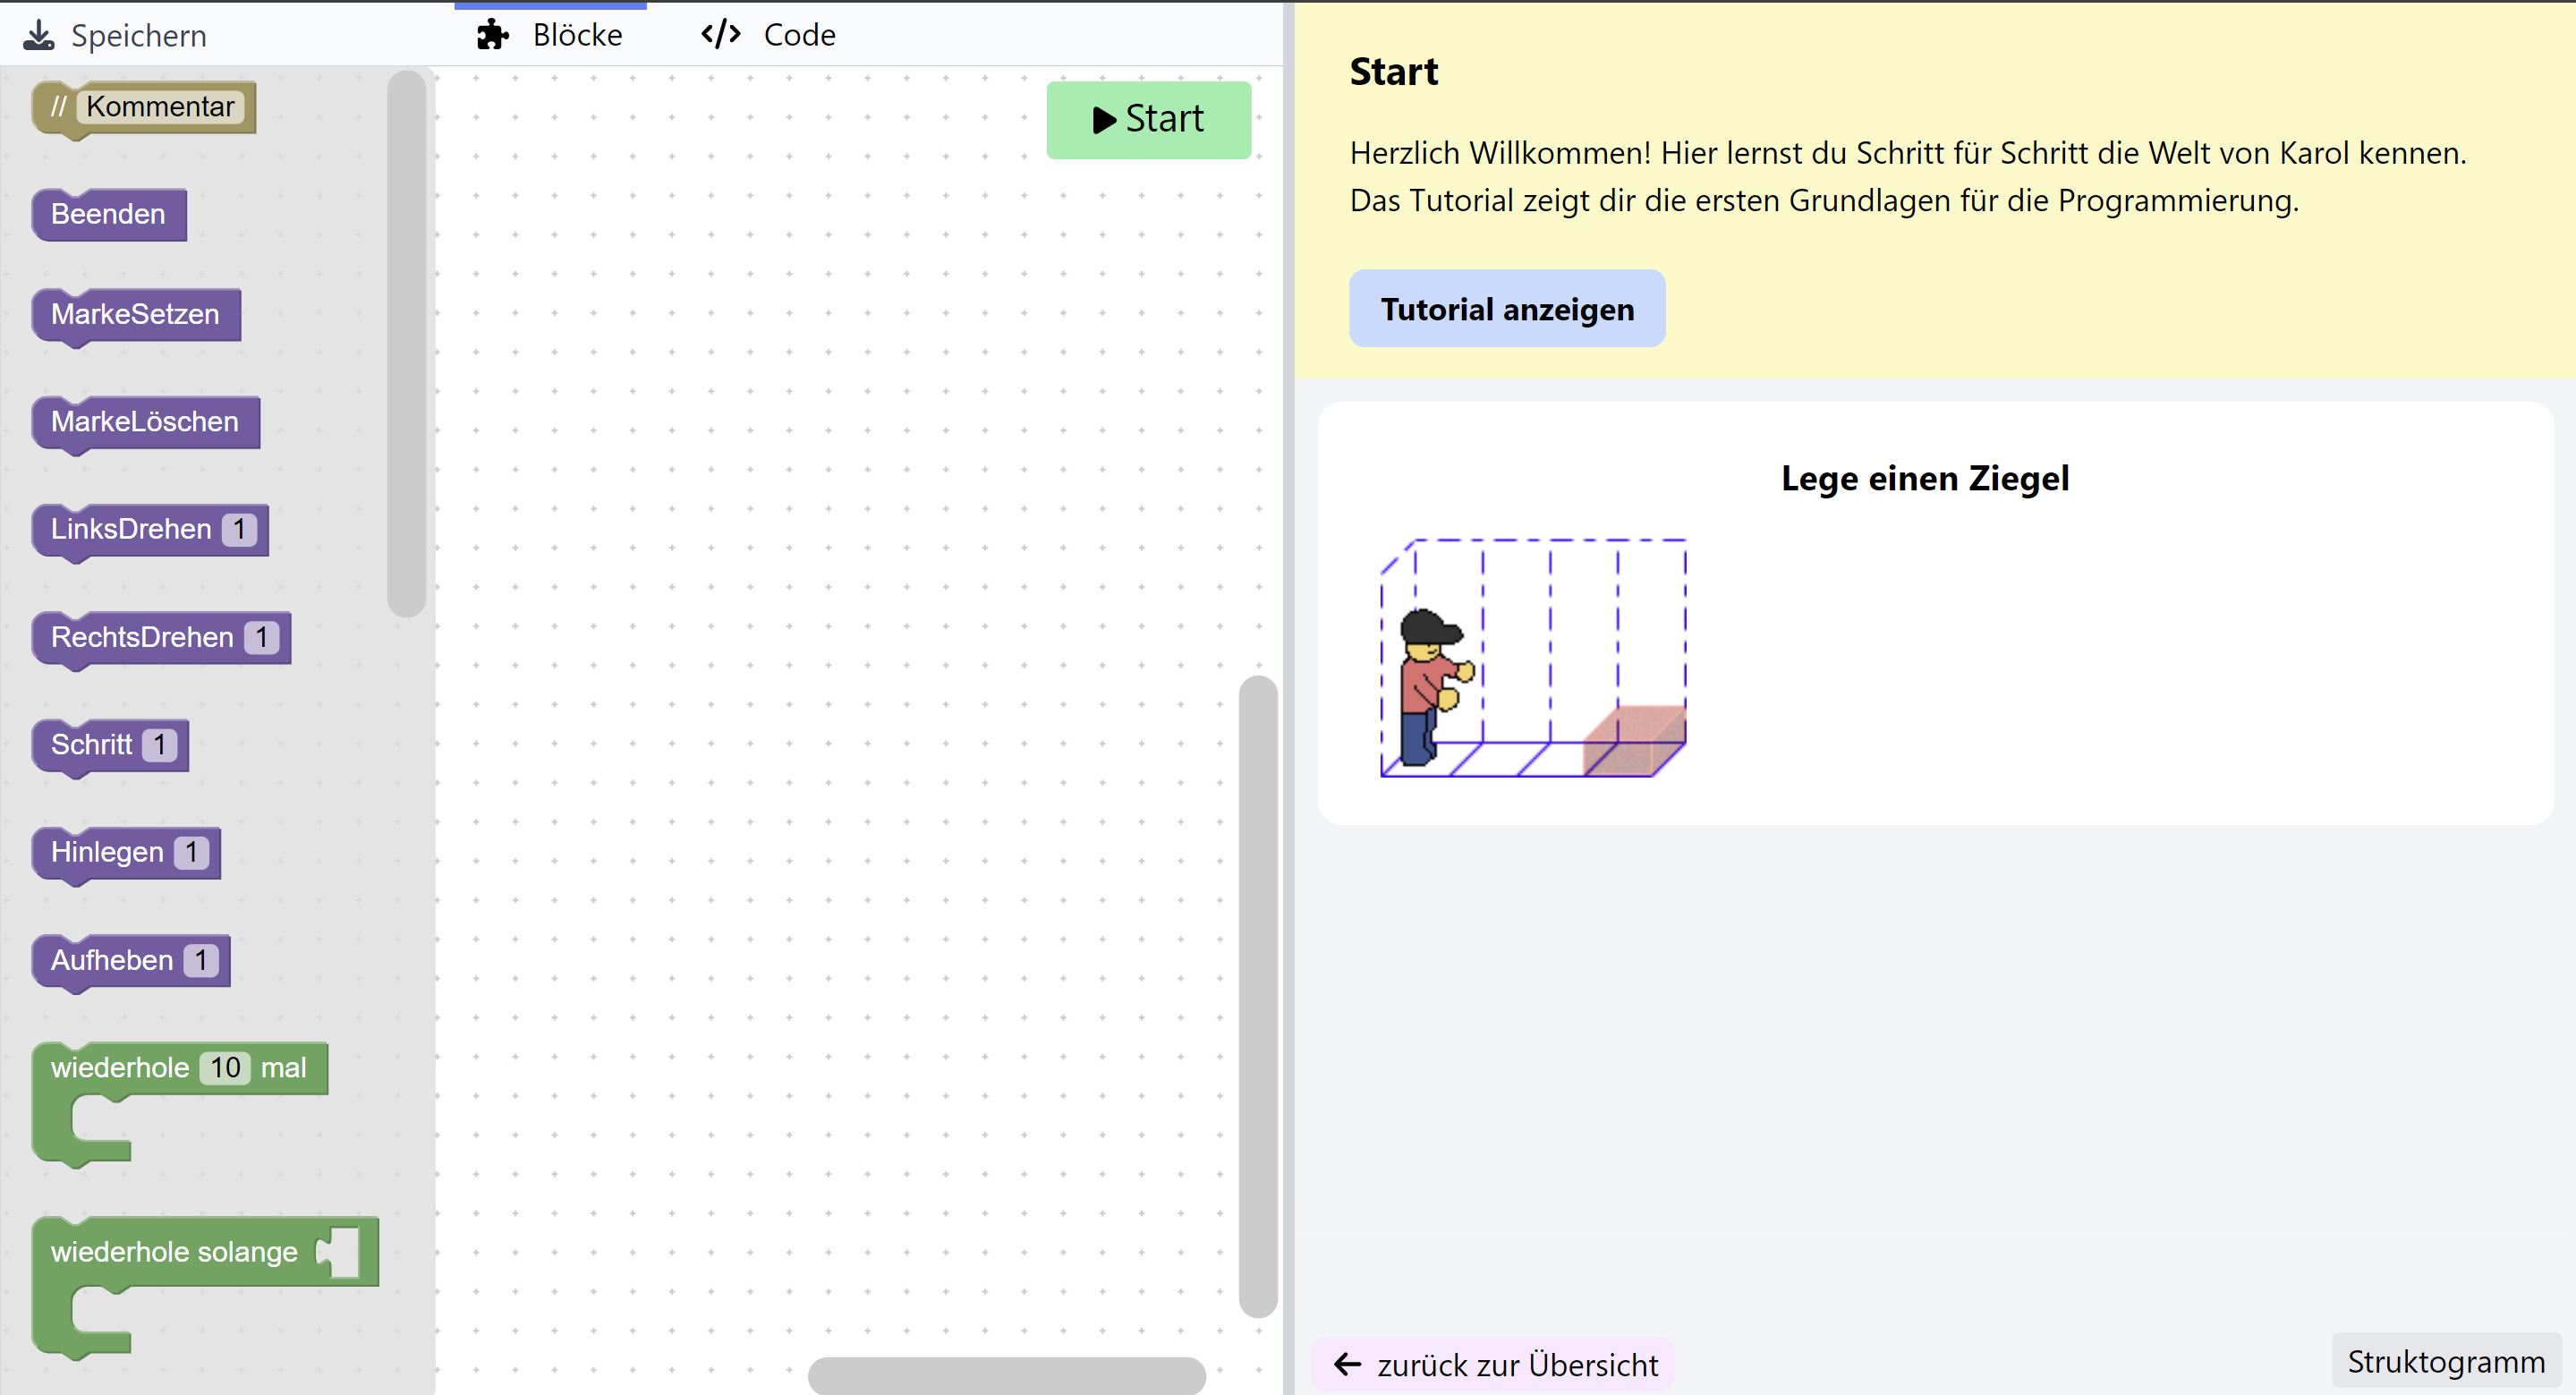
\includegraphics[width=0.85\textwidth]{_Aufgaben/BlocksAndJava/img/overview.png}
\end{center}

\Aufgabe{Karol-Java Übersetzung}{

\begin{enumerate}
    \item Bearbeite die Aufgaben von Robot Karol online: \url{karol.arrrg.de}
    \item Schalte in der Code-Ansicht die Sprache auf Java um und notiere auf dem AB jeweils zu welchem Java-Code der Block übersetzt wird. Achte hierbei auf Einrückungen!
\end{enumerate}


\begin{tabularx}{\textwidth}{p{4cm}X}


\includegraphics[height=25pt]{_Aufgaben/BlocksAndJava/img/step2.png}& \LoesungLine{karol.schritt(2);}{1}\\

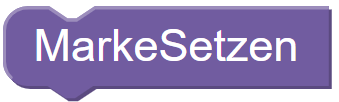
\includegraphics[height=25pt]{_Aufgaben/BlocksAndJava/img/markeSetzen.png}& \LoesungLine{karol.markeSetzen();}{1}\\


\includegraphics[height=25pt]{_Aufgaben/BlocksAndJava/img/step10.png}& \LoesungLine{karol.schritt(10);}{1}\\

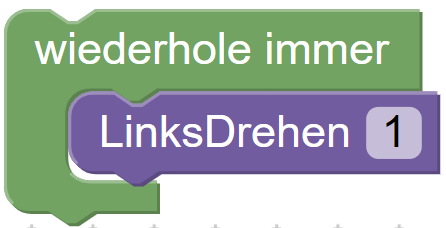
\includegraphics[width=\linewidth]{_Aufgaben/BlocksAndJava/img/whileTrue.png}&
\LoesungLine{while(true) \{ \newline \indent\hspace{1cm} karol.linksDrehen(1); \newline \} }{3}\\

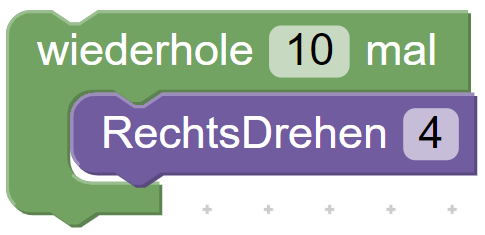
\includegraphics[width=\linewidth]{_Aufgaben/BlocksAndJava/img/for10.png}&\LoesungLine{for(int i=0; i < 10; i++) \{ \newline \indent\hspace{1cm} karol.rechtsDrehen(4); \newline \} }{3}

\end{tabularx}

\begin{tabularx}{\textwidth}{p{6cm}X}

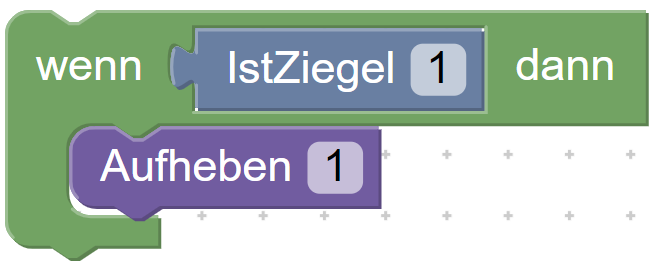
\includegraphics[width=\linewidth]{_Aufgaben/BlocksAndJava/img/if.png}& 
\LoesungLine{if(karol.istZiegel()) \{ \newline \indent\hspace{1cm} karol.aufheben(1); \newline \}}{3}\\\\

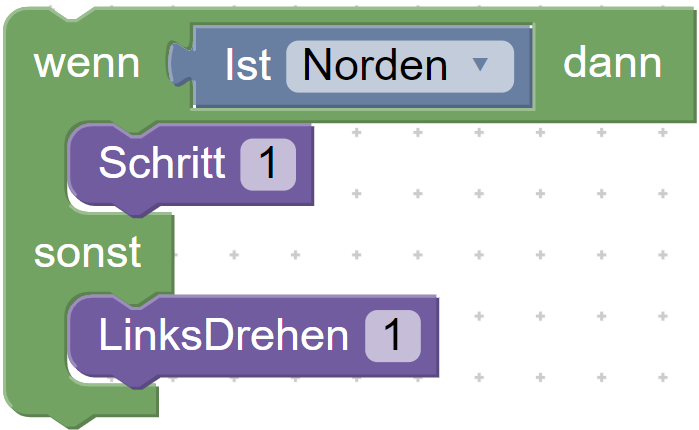
\includegraphics[width=\linewidth]{_Aufgaben/BlocksAndJava/img/ifelse.png}&
\LoesungLine{if(karol.istNordern()) \{ \newline \indent\hspace{1cm} karol.aufheben(1); \newline \} else \{ \newline \indent\hspace{1cm} karol.linksDrehen(1); \newline \}}{5}

\end{tabularx}

}